
\section*{Foreword}
\begin{figure}[ht] 
	
	\centering
	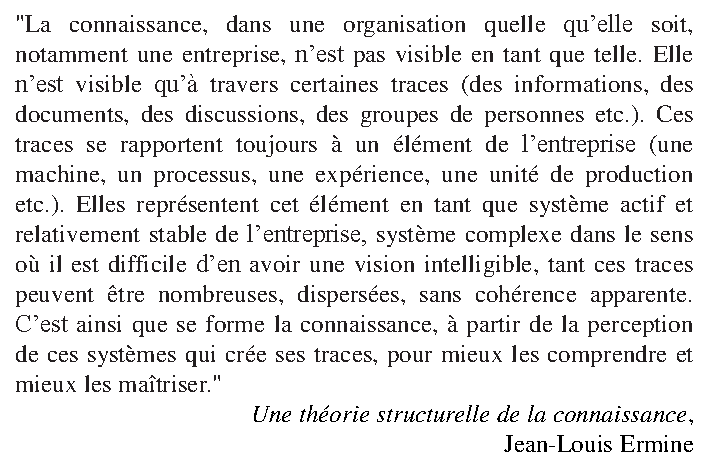
\includegraphics[width=.7\linewidth]{images/citation-ermine.pdf}
\end{figure}



\section{Introduction}
\label{sect:intro}


The purpose of this report is to document the work done as part of the Second Task described in the Convention de l’équipe de recherche commune. This document corresponds to Deliverable 2. The core contribution of this document is a domain-specific language (DSL) for traceability, expressive enough to cover all the potential traceability applications we have discussed during this project. 

More specifically, we include a short reminder of the terminology we use in the DSL, the definition of both the abstract (\textit{i.e.,} metamodel) and concrete syntax (a JSON-based representation), and an Ecore implementation of the DSL in an Eclipse plugin. We illustrate the usability of the DSL with a running example: the transclusion of model elements in certification documents.


%"La connaissance, dans une organisation quelle qu’elle soit, notamment une entreprise, n’est pas visible en tant que telle. Elle n’est visible qu’à travers certaines traces (des informations, des documents, des discussions, des groupes de personnes etc.). Ces traces se rapportent toujours à un élément de l’entreprise (une machine, un processus, une expérience, une unité de production etc.). Elles représentent cet élément en tant que système actif et relativement stable de l’entreprise, système complexe dans le sens où il est difficile d’en avoir une vision intelligible, tant ces traces peuvent être nombreuses, dispersées, sans cohérence apparente. C’est ainsi que se forme la connaissance, à partir de la perception de ces systèmes qui crée ses traces, pour mieux les comprendre et mieux les maîtriser."
